% 第8章第3节：典型方程的解析求解（可分离变量与标量线性方程；常系数线性系统；时变线性系统）。

\section{典型方程的解析求解}
\label{sec:ode-analytic-solutions}

上一节的理论说明解存在、唯一并连续依赖数据，却没有给出解的公式。本节处理能直接算出解的几类方程。每个公式都要同时核对两件事：它满足方程，也满足初值；它在哪个时间区间上成立。一般非线性方程没有闭式解，前一节的理论对它们照样适用，数值方法则在第~\ref{sec:ode-numerics}节处理。

\subsection{可分离变量方程与标量线性方程}
\label{sec:ode-separable-linear}

\paragraph{可分离变量方程}
若标量方程的右端可以写成时间因子与状态因子的乘积，
\begin{equation}
  \dot x=a(t)\,h(x),
  \label{eq:ode-separable}
\end{equation}
其中$a$在区间$I$上连续，$h$在开区间$D$上局部Lipschitz，就称它为可分离变量方程。形式上把$x$都移到一边、$t$移到另一边再积分，就得到解的隐式关系。下面说明这一操作何时合法。

先看$h(x_0)=0$的情形：常值函数$x\equiv x_0$满足方程与初值，由唯一性它就是解。这类解称为平衡解，在形式计算中两边除以$h(x)$时会被丢掉，必须单独列出。

再看$h(x_0)\neq0$的情形。这时解在整个最大存在区间上都满足$h(x(t))\neq0$：若某时刻$t_1$有$h(x(t_1))=0$，则常值函数$x\equiv x(t_1)$与$x$是从$(t_1,x(t_1))$出发的两个解，唯一性要求二者相同，与$h(x_0)\neq0$矛盾。于是$x(t)$始终留在包含$x_0$、使$h\neq0$的那个开区间$D_0$中。在$D_0$上令
\[
  G(x)=\int_{x_0}^x\frac{\mathrm d\xi}{h(\xi)},
\]
$G'=1/h$不变号，所以$G$严格单调。链式法则给出$\frac{\mathrm d}{\mathrm dt}G(x(t))=\dot x/h(x)=a(t)$，从$t_0$积分得
\begin{equation}
  G\bigl(x(t)\bigr)=\int_{t_0}^ta(s)\,\mathrm ds.
  \label{eq:ode-separable-implicit}
\end{equation}
$G$可逆，因此$x(t)=G^{-1}\bigl(\int_{t_0}^ta\bigr)$；这个式子在右端的积分落在$G$的值域内时成立，值域的端点正对应最大存在区间的端点。

\paragraph{时间等于路程除以速度}
取$a\equiv1$，式~\eqref{eq:ode-separable-implicit}变成
\[
  t-t_0=\int_{x_0}^{x(t)}\frac{\mathrm d\xi}{h(\xi)},
\]
即走过一段路程所需的时间等于路程元除以速度再累计。上一节的两个现象都可以从这个积分读出。若$h$在$+\infty$附近增长得足够快，使$\int_{x_0}^{\infty}\mathrm d\xi/h(\xi)<\infty$，解就在有限时间走到无穷远，这就是$\dot x=x^2$的爆炸。另一方面，若$h$在一个零点$x^\ast$附近满足Lipschitz条件，$|h(\xi)|\leq L|\xi-x^\ast|$，则$\int\mathrm d\xi/|h(\xi)|$在$x^\ast$附近像$\int\mathrm d\xi/|\xi-x^\ast|$一样发散，状态永远无法在有限时间到达平衡点，这与唯一性一致。$\dot x=\sqrt{|x|}$的反例恰好相反：$\int_0^1\mathrm d\xi/\sqrt\xi=2$有限，所以从原点出发到达$x=1$只需$2$个单位时间，平衡点可以在有限时间内被离开。

\begin{example}[Logistic方程]
  \label{ex:ode-logistic}
  考虑$\dot x=rx(1-x)$，$r>0$。平衡解是$x\equiv0$与$x\equiv1$。对$x_0\notin\{0,1\}$，部分分式给出$\int\mathrm d\xi/(\xi(1-\xi))=\log|\xi/(1-\xi)|$，式~\eqref{eq:ode-separable-implicit}化为$\log\left|\frac{x(1-x_0)}{x_0(1-x)}\right|=rt$。由于$x(t)$与$x_0$位于同一个$D_0$中，绝对值内的量为正，解出
  \[
    x(t)=\frac{x_0e^{rt}}{1-x_0+x_0e^{rt}}.
  \]
  对$x_0\in(0,1)$，分母恒正，解在全部时间存在并单调趋于$1$。对$x_0>1$，分母在$t=\frac1r\log\frac{x_0-1}{x_0}<0$处为零，所以解在过去某时刻从$+\infty$下来，正向全局存在。对$x_0<0$，分母在$t=\frac1r\log\frac{x_0-1}{x_0}>0$处为零，解在有限时间趋于$-\infty$。同一个公式在三种初值下给出三种存在区间，必须结合初值逐一判断。
\end{example}

隐式关系还可能需要选择分支。方程$\dot x=-t/x$定义在$D=(0,\infty)$上，$x(0)=x_0>0$。分离变量得$x\,\mathrm dx=-t\,\mathrm dt$，积分得$x^2+t^2=x_0^2$，这是一个圆。圆上有两个分支$x=\pm\sqrt{x_0^2-t^2}$，初值$x_0>0$选定上半支。解在$(-x_0,x_0)$上存在；在端点处$x\to0$，正是状态集合的边界，向量场$-t/x$在那里没有定义。圆的下半支是另一个初值问题的解，不能接在上半支后面。

\paragraph{积分因子与常数变易}
标量线性方程
\begin{equation}
  \dot x=-a(t)\,x+b(t),\qquad x(t_0)=x_0,
  \label{eq:ode-scalar-linear}
\end{equation}
其中$a,b$在$I$上连续，可以用积分因子求解。令$A(t)=\int_{t_0}^ta(s)\,\mathrm ds$，乘积法则给出$\frac{\mathrm d}{\mathrm dt}\bigl(e^{A(t)}x(t)\bigr)=e^{A(t)}\bigl(\dot x+a x\bigr)=e^{A(t)}b(t)$，积分后得到
\begin{equation}
  x(t)=e^{-A(t)}x_0+\int_{t_0}^te^{-(A(t)-A(s))}\,b(s)\,\mathrm ds.
  \label{eq:ode-scalar-variation}
\end{equation}
代入$t=t_0$得到初值，对$t$求导可验证方程，所以这确是解；由唯一性也是唯一的解。同一公式也可以这样得到：齐次方程$\dot x=-ax$的解是$Ce^{-A(t)}$，让常数$C$随时间变化，代入原方程得$\dot C=e^{A}b$，再积分。这一做法称为\term{常数变易}（variation of constants）。

式~\eqref{eq:ode-scalar-variation}把解分成两部分。第一项是初值的记忆，被因子$e^{-A(t)}$逐渐抹去；第二项是输入的累计，时刻$s$的输入在时刻$t$只剩下$e^{-(A(t)-A(s))}$的份额。对温度模型，$a\equiv\lambda$，$b=u$，
\[
  x(t)=e^{-\lambda(t-t_0)}x_0+\int_{t_0}^te^{-\lambda(t-s)}u(s)\,\mathrm ds.
\]
可以把它想象成：每一时刻送进的一小份热量$u(s)\,\mathrm ds$都以速率$\lambda$独立地散掉，此刻的温差是所有尚未散尽的份额之和。$\lambda=0.2$时，一份热量的半衰期是$\log2/0.2\approx3.47$分钟。恒定输入$u$下，积分算得$x(t)=u/\lambda+(x_0-u/\lambda)e^{-\lambda(t-t_0)}$：初值的作用消退，输入留下平衡值$u/\lambda$。“初值作用趋零”与“状态趋零”是两回事。

\begin{example}[周期加热的稳态响应]
  \label{ex:ode-periodic-heating}
  取$\lambda=0.2$，加热量在$0.4$上下摆动：$u(t)=0.4+0.2\sin\omega t$。试探形如$x_p(t)=2+\alpha\sin\omega t+\beta\cos\omega t$的解，代入方程并比较$\sin\omega t$与$\cos\omega t$的系数，得$\alpha\omega=-\lambda\beta$与$-\beta\omega=-\lambda\alpha+0.2$，解出
  \[
    \alpha=\frac{0.2\lambda}{\lambda^2+\omega^2},\qquad\beta=-\frac{0.2\omega}{\lambda^2+\omega^2}.
  \]
  所以$x_p(t)=2+\frac{0.2}{\sqrt{\lambda^2+\omega^2}}\sin(\omega t-\phi)$，其中$\phi=\arctan(\omega/\lambda)$。取$\omega=0.5$，振幅为$0.2/\sqrt{0.29}\approx0.371$，相位滞后约$1.19$弧度。一般解是$x_p$加上齐次解：$x(t)=x_p(t)+\bigl(x_0-x_p(0)\bigr)e^{-0.2t}$，其中$x_p(0)=2+\beta\approx1.655$。输入摆动越快，状态的摆动越小、越滞后：房间的热容把快速变化平滑掉了。
\end{example}

\paragraph{解析解作为数值基准}
解析解的价值不只在于给出公式。它让我们能精确核对一条轨迹的每个特征：平衡值、衰减速率、稳态振幅、爆炸时刻。第~\ref{sec:ode-numerics}节比较数值方法时，正是用这些公式算出“真值”，再测量误差随步长的变化；没有可核验的真值，就无法区分方法的误差与方程本身的行为。

\subsection{常系数线性系统}
\label{sec:ode-constant-linear}

\paragraph{矩阵指数}
标量方程$\dot x=ax$的解是$e^{at}x_0$。对向量方程$\dot{\bm x}=\bm A\bm x$，$\bm A\in\mathbb R^{d\times d}$，自然的猜测是用某种“矩阵的指数”代替$e^{at}$。指数函数的幂级数只用到乘法与加法，对方阵同样可以写出。矩阵指数在本书前置各卷中没有建立，这里从定义开始。

\begin{definition}[矩阵指数]
  \label{def:ode-matrix-exponential}
  对方阵$\bm A\in\mathbb R^{d\times d}$，定义\term{矩阵指数}
  \begin{equation}
    e^{\bm A}=\sum_{j=0}^\infty\frac{\bm A^j}{j!}=\bm I+\bm A+\frac{\bm A^2}{2!}+\cdots.
    \label{eq:ode-matrix-exponential}
  \end{equation}
\end{definition}

\begin{theorem}[矩阵指数的基本性质]
  \label{thm:ode-matrix-exponential-properties}
  设$\bm A,\bm B\in\mathbb R^{d\times d}$。
  \begin{enumerate}
    \item 级数~\eqref{eq:ode-matrix-exponential}绝对收敛；$\sum_jt^j\bm A^j/j!$在$t$的每个有界集合上一致收敛。
    \item $\frac{\mathrm d}{\mathrm dt}e^{t\bm A}=\bm Ae^{t\bm A}=e^{t\bm A}\bm A$。
    \item 若$\bm A\bm B=\bm B\bm A$，则$e^{\bm A+\bm B}=e^{\bm A}e^{\bm B}$。特别地，$e^{(t+s)\bm A}=e^{t\bm A}e^{s\bm A}$，并且$e^{t\bm A}$可逆，逆为$e^{-t\bm A}$。
    \item 若$\bm V$可逆，则$e^{\bm V\bm\Lambda\bm V^{-1}}=\bm Ve^{\bm\Lambda}\bm V^{-1}$。
  \end{enumerate}
\end{theorem}

\begin{proof}
  (1)取任一次乘性矩阵范数，例如谱范数，则$\|t^j\bm A^j/j!\|\leq(|t|\|\bm A\|)^j/j!$。右端是收敛的数值级数$e^{|t|\|\bm A\|}$的通项，在$|t|\leq T$上一致地被$(T\|\bm A\|)^j/j!$控制，由Weierstrass判别法得结论。

  (2)逐项求导得到级数$\sum_{j\geq1}t^{j-1}\bm A^j/(j-1)!=\bm A\sum_{i\geq0}t^i\bm A^i/i!$，由(1)它在有界区间上一致收敛，所以逐项求导合法。把$\bm A$提到右边也一样。

  (3)两个绝对收敛级数可以按Cauchy乘积相乘并重排：
  \[
    e^{\bm A}e^{\bm B}=\sum_{n\geq0}\sum_{j+k=n}\frac{\bm A^j\bm B^k}{j!\,k!}
    =\sum_{n\geq0}\frac1{n!}\sum_{j=0}^n\binom nj\bm A^j\bm B^{n-j}
    =\sum_{n\geq0}\frac{(\bm A+\bm B)^n}{n!}.
  \]
  最后一步是二项式展开，只有在$\bm A$与$\bm B$可交换时才成立。$t\bm A$与$s\bm A$可交换，取$s=-t$得$e^{t\bm A}e^{-t\bm A}=e^{\bm0}=\bm I$。

  (4)$(\bm V\bm\Lambda\bm V^{-1})^j=\bm V\bm\Lambda^j\bm V^{-1}$，逐项代入并提出$\bm V$与$\bm V^{-1}$。
\end{proof}

由(2)，$\bm x(t)=e^{(t-t_0)\bm A}\bm x_0$满足$\dot{\bm x}=\bm A\bm x$与初值；线性向量场关于状态全局Lipschitz，所以这就是唯一的解，并且对全部$t\in\mathbb R$存在。性质(3)中的可交换条件不能省略，第~\ref{sec:ode-time-varying-linear}小节会给出反例。

\paragraph{常数变易公式}
加入输入后，方程变为
\begin{equation}
  \dot{\bm x}(t)=\bm A\bm x(t)+\bm B\bm u(t),\qquad\bm x(t_0)=\bm x_0,
  \label{eq:ode-lti}
\end{equation}
其中$\bm B\in\mathbb R^{d\times m}$，$\bm u$局部可积。仿照标量情形，令$\bm z(t)=e^{-t\bm A}\bm x(t)$，乘积法则与性质(2)给出$\dot{\bm z}=e^{-t\bm A}(\dot{\bm x}-\bm A\bm x)=e^{-t\bm A}\bm B\bm u(t)$。积分并乘回$e^{t\bm A}$，得到
\begin{equation}
  \bm x(t)=e^{(t-t_0)\bm A}\bm x_0+\int_{t_0}^te^{(t-s)\bm A}\bm B\bm u(s)\,\mathrm ds.
  \label{eq:ode-lti-variation}
\end{equation}
代入$t=t_0$得初值；对上限求导可验证方程，局部可积输入下验证在几乎处处意义上成立。读法与标量情形相同：初态经过$e^{(t-t_0)\bm A}$传播，每一时刻的输入经过剩余时间$t-s$的传播后累加。

\paragraph{用特征方向读出相图}
$e^{t\bm A}$怎样作用，取决于$\bm A$的特征结构。若$\bm A$可对角化，$\bm A=\bm V\bm\Lambda\bm V^{-1}$，性质(4)给出$e^{t\bm A}=\bm Ve^{t\bm\Lambda}\bm V^{-1}$：把初态在特征向量基下展开，第$i$个坐标独立地乘以$e^{\lambda_it}$。实特征值$\lambda_i<0$的方向按指数收缩，$\lambda_i>0$的方向按指数伸长。一对共轭复特征值$\alpha\pm\mathrm i\beta$（$\beta\neq0$）对应一个二维实不变平面：若特征向量为$\bm v=\bm v_{\mathrm r}+\mathrm i\bm v_{\mathrm i}$，在基$\{\bm v_{\mathrm r},\bm v_{\mathrm i}\}$下$\bm A$的作用是$\begin{bmatrix}\alpha&\beta\\-\beta&\alpha\end{bmatrix}$，其指数为
\[
  e^{\alpha t}\begin{bmatrix}\cos\beta t&\sin\beta t\\-\sin\beta t&\cos\beta t\end{bmatrix},
\]
即一边以角速度$\beta$旋转、一边按$e^{\alpha t}$伸缩。实部决定靠近还是远离，虚部决定转得多快。

并非每个矩阵都有完整的特征向量基。若$\bm A$有Jordan块$\lambda\bm I+\bm N$，$\bm N$是幂零矩阵，则$\lambda\bm I$与$\bm N$可交换，性质(3)给出$e^{t(\lambda\bm I+\bm N)}=e^{\lambda t}\sum_{j<r}t^j\bm N^j/j!$，其中$r$是块的大小。指数因子之外多出了$t$的多项式。Jordan块及其幂中出现的多项式因子可参考\BookChapterRef{chap:linear-analysis}{卷一“谱和奇异值”章}。

图~\ref{fig:ode-phase-portraits}用二维例子把这些情形画出来。除(b)外，各图都是线性化的阻尼摆$\dot x_1=x_2$、$\dot x_2=-x_1-cx_2$，只改变阻尼系数$c$。特征方程$\lambda^2+c\lambda+1=0$给出$\lambda=\bigl(-c\pm\sqrt{c^2-4}\bigr)/2$。$c=2.5$时两个负实根$-0.5,-2$，轨迹不旋转地进入原点，并沿收缩较慢的方向$-0.5$贴近原点，称为稳定结点；$c=0.5$时一对实部为$-0.25$的复根，轨迹螺旋进入，称为稳定焦点；$c=0$时纯虚根$\pm\mathrm i$，轨迹是闭合的椭圆，称为中心；$c=-0.5$（负阻尼，相当于不断注入能量）时螺旋向外，称为不稳定焦点。$c=2$是临界情形：$\lambda=-1$是二重根，但$\bm A+\bm I=\begin{bmatrix}1&1\\-1&-1\end{bmatrix}$不为零而平方为零，只有一个特征方向$(1,-1)$，于是
\[
  e^{t\bm A}=e^{-t}\bigl(\bm I+t(\bm A+\bm I)\bigr)=e^{-t}\begin{bmatrix}1+t&t\\-t&1-t\end{bmatrix},
\]
轨迹都沿这唯一的方向进入原点，称为退化结点。(b)是倒立摆在顶点附近的线性化$\dot x_1=x_2$、$\dot x_2=x_1$，特征值$\pm1$，沿$(1,1)$方向伸长、沿$(1,-1)$方向收缩，称为鞍点。

\begin{figure*}[htbp]
  \centering
  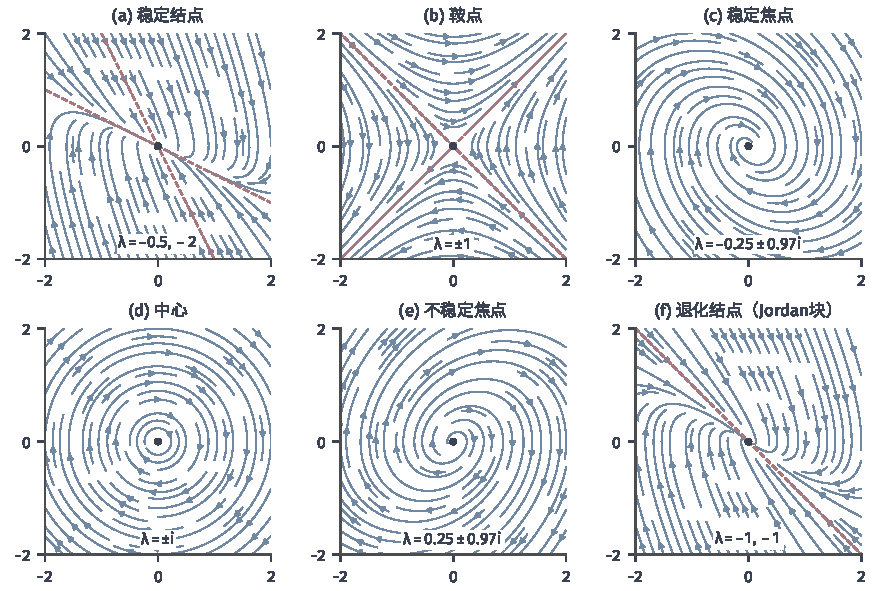
\includegraphics[width=150mm]{figures/03-optimization-evolution-and-signals/02-processes-and-trajectory-evolution/matplotlib/ode-phase-portraits/figure.pdf}
  \caption{二维常系数线性系统$\dot{\bm x}=\bm A\bm x$的相图。(a)(c)(d)(e)(f)取$\bm A=\begin{bmatrix}0&1\\-1&-c\end{bmatrix}$，阻尼系数依次为$c=2.5,0.5,0,-0.5,2$；(b)取$\bm A=\begin{bmatrix}0&1\\1&0\end{bmatrix}$。各图底部标出特征值，红色虚线是实特征向量方向（(f)只有一个）。流线由向量场绘制，箭头表示时间方向。}
  \label{fig:ode-phase-portraits}
\end{figure*}

一般的二阶矩阵可以按迹$\tau=\operatorname{tr}\bm A$与行列式$\Delta=\det\bm A$分类，因为特征值是$\bigl(\tau\pm\sqrt{\tau^2-4\Delta}\bigr)/2$：$\Delta<0$时为鞍点；$\Delta>0$且$\tau^2>4\Delta$时为结点；$\tau^2<4\Delta$时为焦点，$\tau=0$时退化为中心；$\tau^2=4\Delta$是分界情形，由是否可对角化决定是退化结点还是各方向等速收缩的星形结点。稳定与否由$\tau$的符号决定。这些画面在第~\ref{sec:ode-stability}节中用来判断非线性平衡点附近的行为。

\paragraph{分段常值输入下的精确离散}
计算机和控制器通常每隔$h$时间更新一次输入，在两次更新之间保持不变。设$\bm u(t)=\bm u_n$对$t\in[t_n,t_n+h)$成立。把式~\eqref{eq:ode-lti-variation}限制在这一段上，积分中的$\bm u$是常向量，可以提出：
\begin{equation}
  \bm x_{n+1}=\bm A_h\bm x_n+\bm B_h\bm u_n,\qquad
  \bm A_h=e^{h\bm A},\qquad
  \bm B_h=\int_0^he^{r\bm A}\,\mathrm dr\,\bm B,
  \label{eq:ode-zoh}
\end{equation}
其中$\bm x_n=\bm x(t_n)$，积分变量已换成$r=t_n+h-s$。这称为\term{零阶保持离散化}，它在输入确实分段常值时是精确的，与$h$大小无关。若$\bm A$可逆，$\int_0^he^{r\bm A}\,\mathrm dr=\bm A^{-1}(e^{h\bm A}-\bm I)$；$\bm A$奇异时应保留积分形式，或用分块矩阵一次算出两者：
\[
  \exp\left(h\begin{bmatrix}\bm A&\bm B\\\bm0&\bm0\end{bmatrix}\right)=\begin{bmatrix}\bm A_h&\bm B_h\\\bm0&\bm I\end{bmatrix}.
\]
这个等式的理由是：增广状态$(\bm x,\bm u)$满足$\dot{\bm x}=\bm A\bm x+\bm B\bm u$、$\dot{\bm u}=\bm0$，它在$h$时间后的状态既可以用分块矩阵的指数表示，也可以由式~\eqref{eq:ode-zoh}表示。

对温度模型，$\bm A=-\lambda$，$\bm B=1$，于是$a=e^{-\lambda h}$，$b=(1-e^{-\lambda h})/\lambda$。$\lambda=0.2$、$h=1$时$a\approx0.8187$，$b\approx0.9063$。冻结斜率的Euler近似则给出$a=1-\lambda h=0.8$，$b=h=1$。图~\ref{fig:ode-zoh-euler}取$h=2$以放大差别：前$10$分钟加热$0.4$，随后停止。精确离散的点（$a=e^{-0.4}\approx0.6703$，$b\approx1.6484$）恰好落在连续解上，$t=10$时都是$1.7293$；Euler的点（$a=0.6$，$b=2$）在加热阶段偏高，$t=10$时为$1.8445$，停止加热后又衰减过快，$t=20$时为$0.1434$，而真值是$0.2340$。

\begin{figure}[htbp]
  \centering
  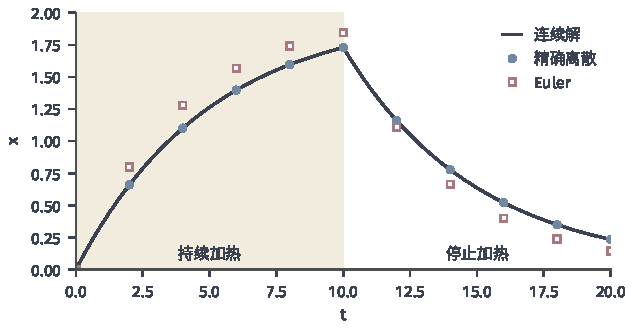
\includegraphics[width=107mm]{figures/03-optimization-evolution-and-signals/02-processes-and-trajectory-evolution/matplotlib/ode-zoh-euler/figure.pdf}
  \caption{分段常值输入下的精确离散与Euler近似。温度模型$\dot x=-0.2x+u$，$x(0)=0$，$u=0.4$（$0\leq t<10$，浅黄底）与$u=0$（$t\geq10$）。黑线为连续解；蓝点为步长$h=2$的零阶保持离散$x_{n+1}=e^{-0.4}x_n+1.6484\,u_n$，与连续解在采样时刻重合；红色方框为同一步长的Euler近似$x_{n+1}=0.6x_n+2u_n$。}
  \label{fig:ode-zoh-euler}
\end{figure}

反过来，从一个离散系数不能唯一推出连续模型。若已知离散模型$x_{n+1}=0.8x_n+u_n$，并把它看作步长$h=1$的Euler近似，对应$\lambda=0.2$、输入增益$1$；若看作零阶保持的精确采样，则需$e^{-\lambda}=0.8$，即$\lambda\approx0.2231$，而输入增益$\beta$须满足$\beta(1-0.8)/0.2231=1$，即$\beta\approx1.116$。两种解释给出不同的连续系统；若步长也未知，可能的连续模型还有无穷多个。此外，零阶保持的精确性依赖“输入在区间内不变”的约定；若真实输入在区间内线性变化，同样的$\bm A_h,\bm B_h$就不再精确。

\subsection{时变线性系统}
\label{sec:ode-time-varying-linear}

\paragraph{状态转移矩阵}
若系数随时间变化，$\dot{\bm x}=\bm A(t)\bm x$，标量情形的积分因子$e^{-\int a}$不能直接推广，原因稍后说明。可以换一个思路：不求公式，而把演化映射本身当作未知量。线性方程的演化映射是线性的，可以用矩阵表示。

\begin{definition}[状态转移矩阵]
  \label{def:ode-state-transition-matrix}
  设$\bm A:I\to\mathbb R^{d\times d}$连续。对$s\in I$，矩阵值函数$t\mapsto\bm\Phi(t,s)$若满足
  \begin{equation}
    \partial_t\bm\Phi(t,s)=\bm A(t)\bm\Phi(t,s),\qquad\bm\Phi(s,s)=\bm I,
    \label{eq:ode-state-transition}
  \end{equation}
  称为$\dot{\bm x}=\bm A(t)\bm x$的\term{状态转移矩阵}。
\end{definition}

$\bm\Phi(t,s)$的第$j$列是从$\bm x(s)=\bm e_j$出发的解，线性方程满足定理~\ref{thm:ode-global-existence}的增长条件，所以这些解在整个$I$上存在且唯一。由线性叠加，从任意$\bm x(s)=\bm\xi$出发的解是$\bm\Phi(t,s)\bm\xi$，即$\bm\Phi(t,s)$就是演化映射$\bm\varphi_{t,s}$的矩阵。

\begin{theorem}[状态转移矩阵的性质]
  \label{thm:ode-state-transition-properties}
  设$\bm A$与$\bm b$在$I$上连续。对$r,s,t\in I$：
  \begin{enumerate}
    \item $\bm\Phi(t,r)\bm\Phi(r,s)=\bm\Phi(t,s)$，并且$\bm\Phi(t,s)$可逆，$\bm\Phi(t,s)^{-1}=\bm\Phi(s,t)$；
    \item $\det\bm\Phi(t,s)=\exp\int_s^t\operatorname{tr}\bm A(\tau)\,\mathrm d\tau$；
    \item $\dot{\bm x}=\bm A(t)\bm x+\bm b(t)$、$\bm x(t_0)=\bm x_0$的解为
    \begin{equation}
      \bm x(t)=\bm\Phi(t,t_0)\bm x_0+\int_{t_0}^t\bm\Phi(t,s)\bm b(s)\,\mathrm ds.
      \label{eq:ode-ltv-variation}
    \end{equation}
  \end{enumerate}
\end{theorem}

\begin{proof}
  (1)是定理~\ref{thm:ode-evolution-composition}的矩阵形式：两边都是在时刻$r$等于$\bm\Phi(r,s)$的解。取$t=s$得$\bm\Phi(s,r)\bm\Phi(r,s)=\bm I$。

  (2)记$\bm\Phi(t)=\bm\Phi(t,s)$，$\delta(t)=\det\bm\Phi(t)$。行列式对每一行线性，所以$\dot\delta$等于把第$i$行换成其导数后的$d$个行列式之和。由$\dot{\bm\Phi}=\bm A\bm\Phi$，$\bm\Phi$第$i$行的导数是$\sum_kA_{i,k}(t)\times(\text{第}k\text{行})$；换入后，$k\neq i$的项含两个相同的行，行列式为零，只剩$A_{i,i}\delta$。求和得$\dot\delta=\operatorname{tr}\bm A(t)\,\delta$，$\delta(s)=1$，解这个标量线性方程即得结论。

  (3)对式~\eqref{eq:ode-ltv-variation}求导，积分上限给出$\bm\Phi(t,t)\bm b(t)=\bm b(t)$，被积函数对$t$求导给出$\bm A(t)\bm\Phi(t,s)\bm b(s)$，合起来是$\bm A(t)\bm x(t)+\bm b(t)$；代入$t=t_0$得初值。
\end{proof}

性质(2)称为Liouville公式，它把体积的变化与向量场的迹联系起来，第~\ref{sec:ode-flows}小节的面积计算和第~\ref{sec:ode-hamiltonian}节的体积保持都要用到它。它也说明$\bm\Phi(t,s)$总是可逆，与性质(1)一致。

\paragraph{时间次序不能交换}
标量情形$\Phi(t,s)=\exp\int_s^ta$，自然要问矩阵情形是否有$\bm\Phi(t,s)=\exp\int_s^t\bm A$。一般没有。取两个常矩阵
\[
  \bm A_1=\begin{bmatrix}0&1\\0&0\end{bmatrix},\qquad\bm A_2=\begin{bmatrix}0&0\\1&0\end{bmatrix},
\]
在$[0,1)$上$\bm A(t)=\bm A_1$，在$[1,2]$上$\bm A(t)=\bm A_2$（分段连续的系数，转移矩阵仍由分段求解拼接得到）。先运行$\bm A_1$一单位时间，再运行$\bm A_2$一单位时间，实际的传播是
\[
  \bm\Phi(2,0)=e^{\bm A_2}e^{\bm A_1}=\begin{bmatrix}1&0\\1&1\end{bmatrix}\begin{bmatrix}1&1\\0&1\end{bmatrix}=\begin{bmatrix}1&1\\1&2\end{bmatrix}.
\]
而$\int_0^2\bm A=\bm A_1+\bm A_2=\begin{bmatrix}0&1\\1&0\end{bmatrix}$，其指数为$\begin{bmatrix}\cosh1&\sinh1\\\sinh1&\cosh1\end{bmatrix}\approx\begin{bmatrix}1.543&1.175\\1.175&1.543\end{bmatrix}$，与真实传播不同。把顺序倒过来，$e^{\bm A_1}e^{\bm A_2}=\begin{bmatrix}2&1\\1&1\end{bmatrix}$又是第三个结果。几何上，$e^{\bm A_1}$是水平剪切，$e^{\bm A_2}$是竖直剪切，先做哪个会得到不同的形变；积分$\int\bm A$把整段时间的系数加在一起，丢掉了先后次序。

若对全部$t,s$都有$\bm A(t)\bm A(s)=\bm A(s)\bm A(t)$，次序就无关紧要，此时$\bm\Phi(t,s)=\exp\int_s^t\bm A$。理由是$\bm M(t)=\int_s^t\bm A$与它的导数$\bm A(t)$可交换，所以$\frac{\mathrm d}{\mathrm dt}\bm M^j=j\bm M^{j-1}\bm A(t)$，逐项求导得$\frac{\mathrm d}{\mathrm dt}e^{\bm M(t)}=\bm A(t)e^{\bm M(t)}$。标量方程和形如$\bm A(t)=a(t)\bm A_0$的系数都属于这种情形。

\paragraph{传播矩阵的计算与受迫响应}
除了可交换等特殊结构，$\bm\Phi(t,s)$一般没有闭式表达，需要求解$d\times d$个分量的矩阵初值问题~\eqref{eq:ode-state-transition}。是否值得这样做，取决于要回答的问题。若只要一条给定输入下的轨迹，直接对$\dot{\bm x}=\bm A(t)\bm x+\bm b(t)$作数值积分即可，只需一个$d$维初值问题。若要比较许多不同输入下的响应，或者要知道时刻$s$的一个单位脉冲在时刻$t$留下多少，就需要$\bm\Phi(t,s)$本身；对输出$\bm y=\bm C(t)\bm x$，式~\eqref{eq:ode-ltv-variation}说明输入到输出的历史核是$\bm C(t)\bm\Phi(t,s)\bm B(s)$，常系数时化为只依赖时间差的$\bm Ce^{(t-s)\bm A}\bm B$。

举一个可交换的例子：通风强度按一天的节律变化，散热系数为$\lambda(t)=0.2+0.1\sin(2\pi t/T_{\mathrm{day}})$。标量情形总可交换，$\Phi(t,s)=\exp\bigl(-\int_s^t\lambda\bigr)$，于是受迫响应$\int_{t_0}^t\Phi(t,s)u(s)\,\mathrm ds$中，同一份热量在通风强的时段散失得快、弱的时段散失得慢。一旦状态是多维的，并且各时刻的耦合矩阵不可交换，例如两个房间之间的换热随时间以不同方式改变，就只能数值地求$\bm\Phi$。

\paragraph{加权历史投影}
常系数与时变线性系统有一个重要用途：用有限维状态概括一整段输入历史。回到温度模型，取$x(0)=0$，常数变易公式给出
\[
  x(t)=\int_0^te^{-\lambda(t-s)}u(s)\,\mathrm ds.
\]
从另一个角度看，$x(t)$是输入历史在权函数$e^{-\lambda(t-s)}$下的加权累计，也就是历史在常数函数上的一个加权投影系数。它满足一个一维的微分方程，所以只用一个数就能随时更新这项历史特征。自然的问题是：若要保留更多的历史特征，例如加权平均之外的“趋势”，相应的系数能否仍然组成一个闭合的线性状态方程？

一般地，设要保留的系数为$c(t)=\int_{\alpha(t)}^{t}u(s)\psi(t,s)\,\mathrm ds$，其中$\psi$是基函数与权函数的乘积，积分窗口的左端$\alpha(t)$可以随时间移动。在$\psi$及其偏导数连续时，对上下限和被积函数求导的Leibniz法则给出
\begin{equation}
  \dot c(t)=u(t)\psi(t,t)-\dot\alpha(t)\,u\bigl(\alpha(t)\bigr)\psi\bigl(t,\alpha(t)\bigr)+\int_{\alpha(t)}^tu(s)\,\partial_t\psi(t,s)\,\mathrm ds.
  \label{eq:ode-history-leibniz}
\end{equation}
三项分别来自新输入进入窗口、旧输入离开窗口，以及窗口内部权重或基函数随时间改变。要得到闭合的状态方程，需要两点：第三项中的$\partial_t\psi$能写成已保留的基函数的线性组合；第二项要么不出现，要么能用已有系数表示。

\begin{example}[指数权下的闭合历史状态]
  \label{ex:ode-laguerre-history}
  取从$0$开始不断增长的窗口（$\alpha\equiv0$），以及基函数$\psi_k(t,s)=\frac{(t-s)^k}{k!}e^{-\lambda(t-s)}$，$k=0,1,\ldots,K-1$。令$c_k(t)=\int_0^tu(s)\psi_k(t,s)\,\mathrm ds$。由于$\psi_k(t,t)$在$k=0$时为$1$、$k\geq1$时为$0$，并且$\partial_t\psi_k=\psi_{k-1}-\lambda\psi_k$（$k\geq1$），$\partial_t\psi_0=-\lambda\psi_0$，式~\eqref{eq:ode-history-leibniz}给出
  \[
    \dot c_0=-\lambda c_0+u,\qquad\dot c_k=-\lambda c_k+c_{k-1}\quad(k\geq1).
  \]
  这是常系数线性系统$\dot{\bm c}=\bm A\bm c+\bm e_1u$，$\bm A=-\lambda\bm I+\bm N$，其中$\bm N$只在主对角线下方一条为$1$，所以$\bm A$恰是一个$K\times K$的Jordan块的转置。截断到前$K$项，方程仍然精确闭合：系数$c_0,\ldots,c_{K-1}$本身没有误差。误差只出现在用有限个系数重建输入历史的时候。
\end{example}

均匀权重的滑动窗口则不闭合。取窗口长度$T$，$c_0(t)=\frac1T\int_{t-T}^tu(s)\,\mathrm ds$，式~\eqref{eq:ode-history-leibniz}给出$\dot c_0=\bigl(u(t)-u(t-T)\bigr)/T$，需要$T$时间以前的输入值，而它不是任何已保留系数的函数。要精确地更新，就得保存整段窗口；有限维状态只能用已有系数重建出的近似值代替$u(t-T)$，这一步引入的余项不会因为系数方程是线性的而消失。

高阶多项式投影（high-order polynomial projection operators, HiPPO）框架系统地研究这类构造\scite{gu2020hippo}。其中一种取法把$[0,t]$上的均匀测度与缩放到$[0,t]$上的Legendre多项式作为权与基，得到时变线性方程$\dot{\bm c}=-\frac1t\bm A\bm c+\frac1t\bm Bu$，其中$A_{n,k}=\sqrt{2n+1}\sqrt{2k+1}$（$n>k$），$A_{n,n}=n+1$，$A_{n,k}=0$（$n<k$），$B_n=\sqrt{2n+1}$。它在截断后仍然闭合，原因与示例~\ref{ex:ode-laguerre-history}相同：基函数关于$t$的导数落在次数不更高的多项式张成的空间里。各时刻的系数矩阵都是同一个$\bm A$的倍数，彼此可交换，所以由上一段的结论，状态转移矩阵为$\bm\Phi(t,s)=\exp\bigl(-\log(t/s)\,\bm A\bigr)$。这里的$\tfrac1t$在$t=0$处奇异，初始状态须另行规定。投影坐标保存哪些历史特征由窗口、权和基共同决定；有限个系数逼近历史的误差、更新方程是否闭合，以及离散实现对扰动是否稳定，是三件需要分别核对的事。数值离散这些方程的方法统一放在第~\ref{sec:ode-numerics}节。
